\documentclass[notitlepage]{report}
\usepackage{graphicx}
\usepackage[left=1in, right=1in, top=1in, bottom=1in]{geometry}
\usepackage{titling}
\usepackage{lipsum}
\pretitle{\begin{center}\Huge\bfseries}
\posttitle{\par\end{center}\vskip 0.5em}
\preauthor{\begin{center}\Large\ttfamily}
\postauthor{\end{center}}
%\predate{\par\large\centering}
%\postdate{\par}
\title{Higher-order Combinations of Existing Ideas}
\author{Us and others}
%\date{\today}
\date{}
\begin{document}
\maketitle
\thispagestyle{empty}
Sir:\\

Co-citation, when two articles are cited by a third, represents the combination of two existing ideas into a third. The frequency of co-citation, which accumulates over time, represents the extent to which this idea is considered by the research community. Marshakova-Shaikevich and Small independently described co-citation in 1973, emphasizing its forward looking characteristics compared to bibliographic coupling.  Co-citation measurements have since been extensively used in scientometrics for a variety of purposes.

From a sampling of the physics literature, Small reported 4 pairs of articles with a co-citation frequency of 49 and greater. The volume of scientific literature has grown considerably since; more co-cited pairs have been discovered; frequencies have increased; and the scale of studies has become larger. Improved bibliographies and modern computing tools have also rendered co-citation calculations relatively facile. 

Uzzi et al. reported a study on novelty in which they examined co-cited references from roughly 18 million articles. Devarakonda et al. reported that 1,309 of 33.6 million co-cited pairs derived from articles published in Scopus in the years 1985--1995 had co-citation frequencies of over 1,000. More recently, Zhao et al. have computed co-citation frequencies for 940 million co-cited article pairs from the same period and identified roughly 1,200 pairs with delayed kinetics analogous to Sleeping Beauty publications. 

A natural extension of co-citation theory is document coupling of a higher order, for example, triads, tetrads, and greater. Triads, for example, can be viewed as either the coming together of three previously independent ideas or the coalescence of three overlapping co-citations in the triad. Indeed, Small proposed a model of multiple citation in 1974 in which tri-citations measured in a set of 6 publications. In his report, Small used intersections of sets of citing papers to measure co-citation frequency, `If $A$ is the set of papers citing document $a$, and $B$ the set citing $b$,the frequency of co-citation of $a$ and $b$ is $n(A \cap B)$'.

An alternate way of looking at these patterns is to view any article $A$ that cites $n$ articles as being composed of $n$ citations, $n\choose2$ co-citations, $n\choose3$ tri-citations etc. Calculating the frequencies of these combinations in a bibliography is relatively expensive, however. An article with either 25 or 50 cited references represents 300 or 1,225 co-citations respectively. The same article also consists of  2,300 or 19,600 tri-citations and  12,650 or  230,300 tetra-citations. For evena modestly sized collection of 2 million articles with an average of 30 references each, this could involve computing $8.12\times10^9$ tri-citations, $5.48\times10^{10}$ tetra-citations, or $2.85\times10^{11}$ penta-citations.  However, scalable and affordable computing today places measuring these higher order assemblies within reach of the scientometrist, and may open a new frontier for discovery

In an initial exploration of higher-order combinations, we have used a `brute force' approach to compute triad frequencies from an 11-year dataset of articles in the Scopus bibliography to identify 181 million triads that are tri-cite d between 1 and 13,000 times. 

In illustration, we discuss an example with a tri-citation frequency of 13,000 (the highest that we observed) originating from the field of physical chemistry. Its component co-cited pairs have been co-cited 16,000, 25,000, and 52,000 times, and the individual articles in this triad have been cited 38,000, 72,000, and 75,000 times respectively (Figure 1).All  three articles in this triad relate to density functional theory and represent methods papers that develop out of the work of Kohn and Pople (need to check if it should be only Kohn).

\begin{figure}[h!]
\begin{center}
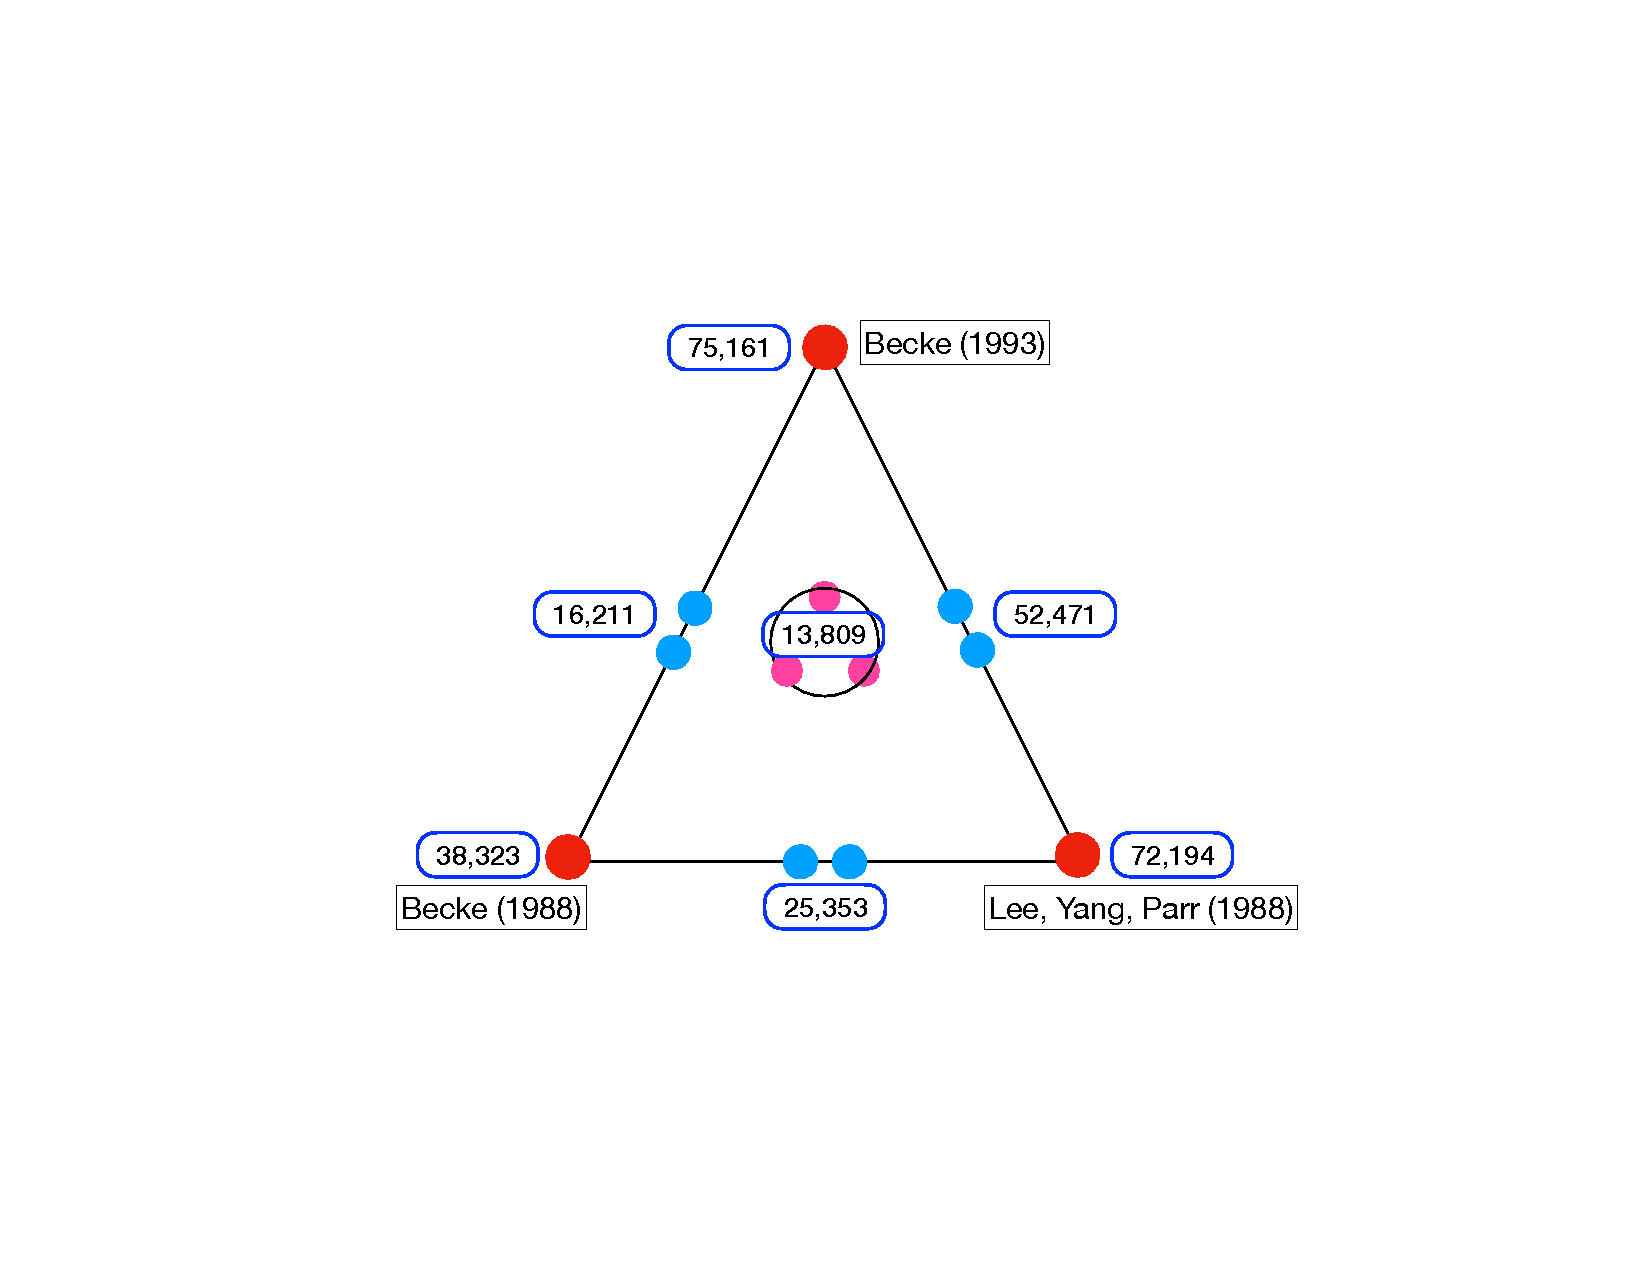
\includegraphics[width=10cm]{fig1.pdf}% This is a *.eps file
\end{center}
\caption{A high frequency triplet. The triad of (i) Becke (1988), (ii) Becke (1992), and (iii) Lee, Yang, and Parr (1988).  Frequencies (round rectangles with blue borders) are shown for the tri-citation (center of triangle), co-citations (sides of triangle), and 
article citations (vertices of triangle). 
}
\label{fig:fig2}
\end{figure}


\emph{This is where we insert get Henry's initial thoughts. maybe Kennie Merz would be interested in joining in}

\end{document}